\documentclass[parskip,10pt,abstracton]{scrartcl}
\usepackage[top=3cm, bottom=3cm, left=3cm, right=3cm]{geometry}
\usepackage{polyglossia}
\setmainlanguage{german}
\pagenumbering{gobble}

\usepackage{setspace}
\onehalfspacing

% ------------------------------------------------------------------------------------
% packages
\usepackage{graphicx}
\usepackage{tikz}
\usetikzlibrary{arrows,shapes,positioning, shadows,trees}
\usepackage{enumerate}

% ------------------------------------------------------------------------------------
% Header
% ------------------------------------------------------------------------------------
\renewcommand*{\maketitle}{%
	{\centering\LARGE\sffamily\bfseries Aufgabe 3: Strukturierung der Nutzeroberfläche \par}
	\vspace{3em}
}

% ====================================================================================
% Document
% ====================================================================================
\begin{document}

\maketitle

% ------------------------------------------------------------------------------------
\section*{Entwurf 1} % Chris 1

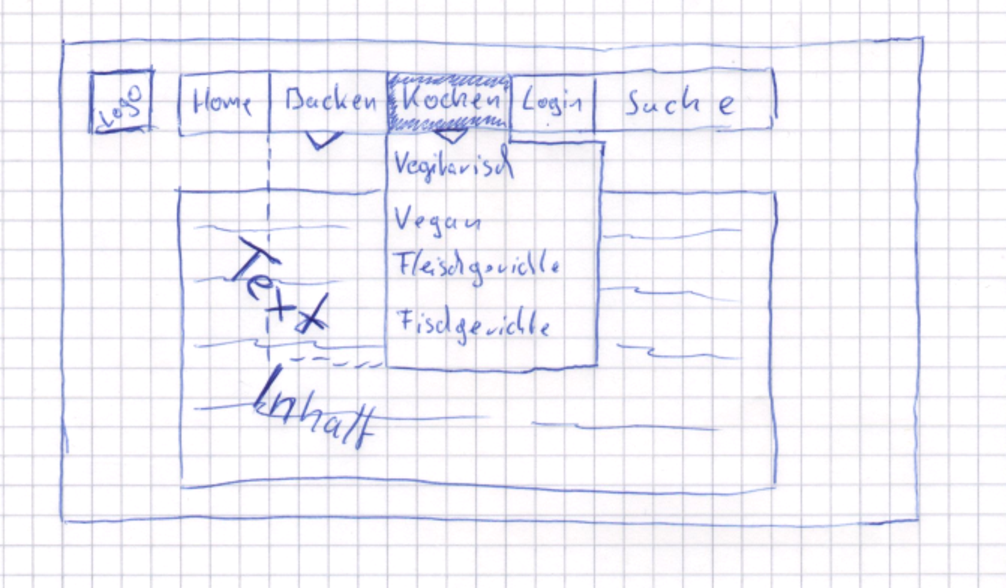
\includegraphics[scale=0.8]{Entwürfe/Chris/chris1.pdf}


Vorteile: \\
- einfach und übersichtlich\\
- Seite nicht überladen

Nachteile: \\
- Menüpunkte Backen/Kochen können unübersichtlich werden bei zu vielen Unterkategorien\\
- unklar, was Login beinhaltet (welche Funktionen hat man davon?) -> Hinweis auf persönliche Funktionen / Möglichkeiten

% ------------------------------------------------------------------------------------
\section*{Entwurf 2} % Chris 2

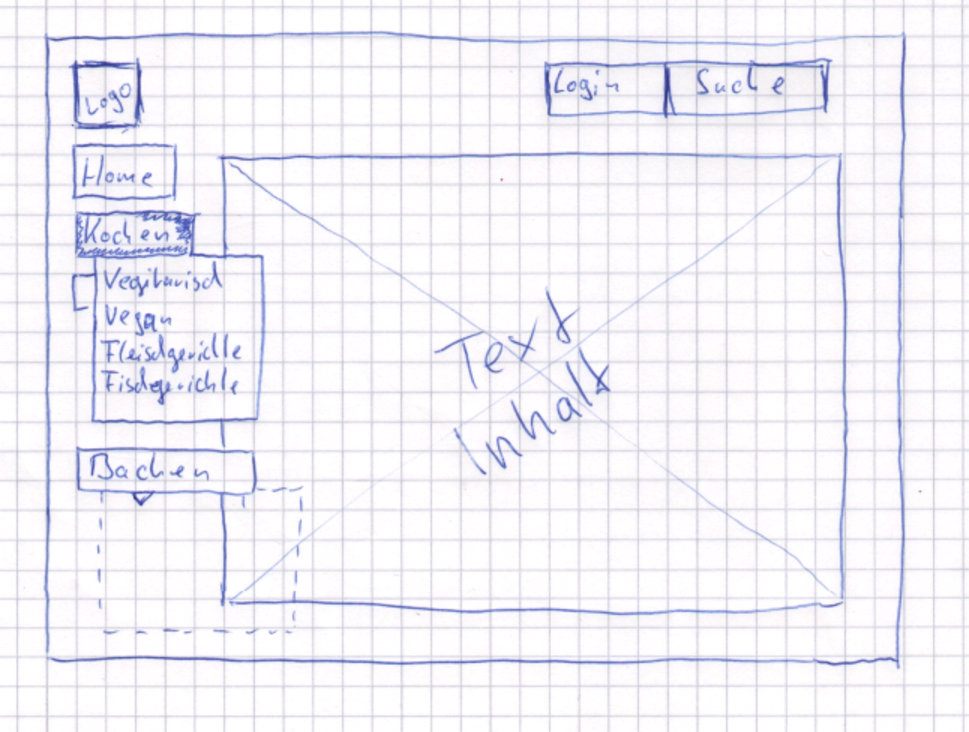
\includegraphics[scale=0.8]{Entwürfe/Chris/chris2.pdf}

Vorteile:\\
- klassischer Aufbau und daher intuitives Zurechtfinden möglich (Position von Login und Suche) \\
- übersichtliches Menü, das sich anpasst (kann klein und groß sein, je nach Bedarf)
-

Nachteile:\\
- Seitenmenü kann problematisch werden, wenn Menüpunkte zu lang sind.


% ------------------------------------------------------------------------------------
\section*{Entwurf 3} % Velat 1

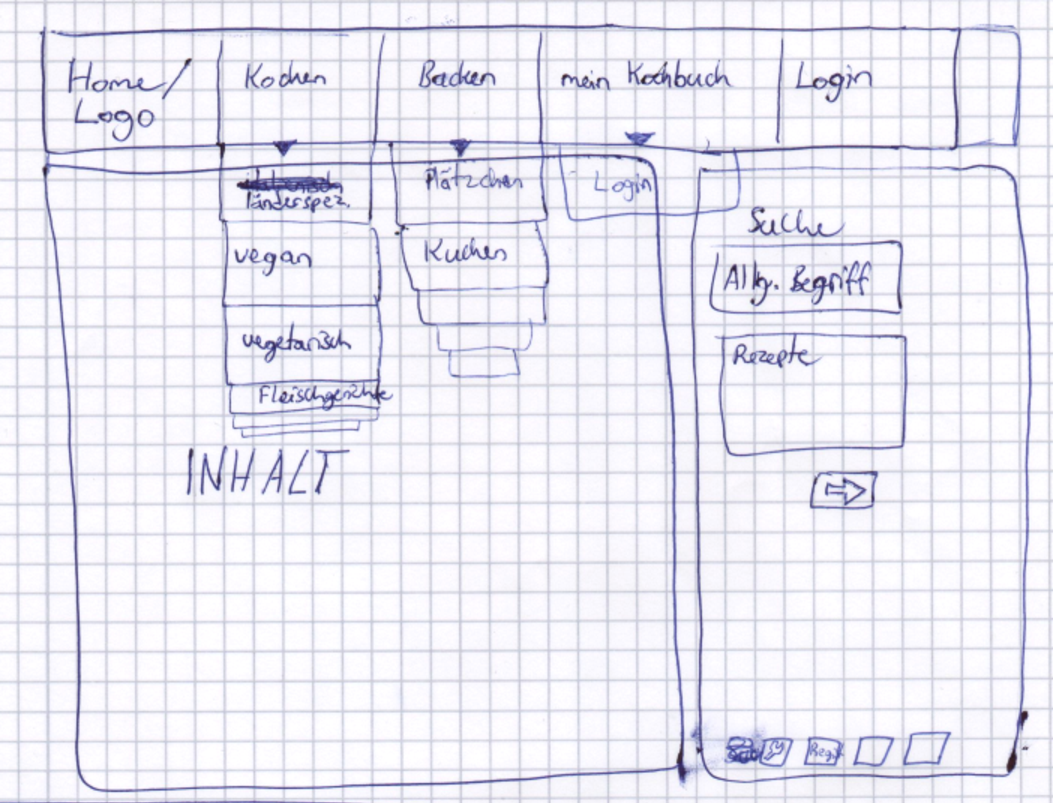
\includegraphics[scale=0.8]{Entwürfe/Velat/velat1.pdf}


Vorteile:\\
- es ist ersichtlich, dass es einen eigenen Kochbuchbereich gibt, für den man sich einloggen muss.
- innovativer Suchbereich
- Suchbereich als eigener Frame jederzeit sichtbar


Nachteile:\\
- Menüpunkte haben zu viele Unterpunkte im Dropdownmenü
- Suchbereich verbraucht Platz von Inhaltsseite
- Suchfunktion zu kompliziert

% ------------------------------------------------------------------------------------
\section*{Entwurf 4} % Velat 2

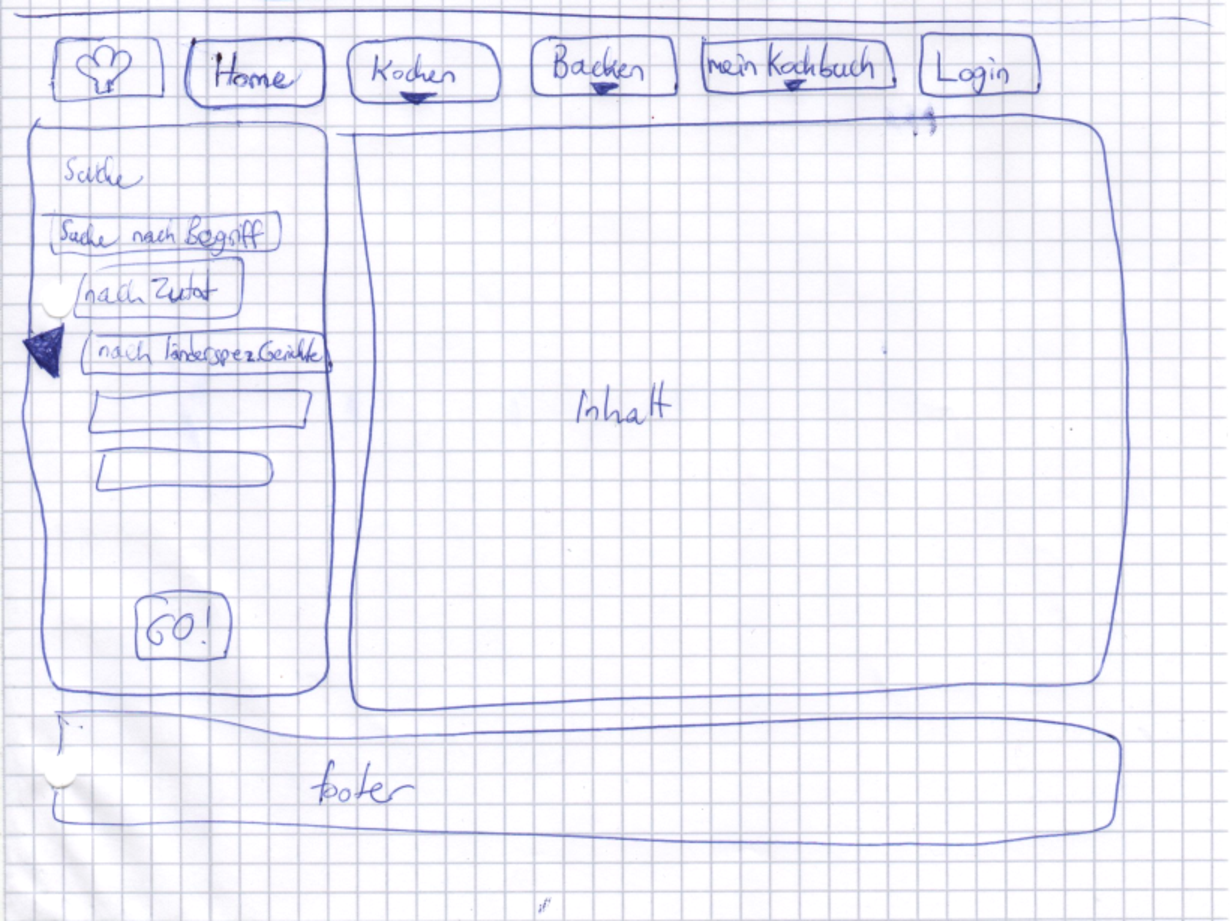
\includegraphics[scale=0.8]{Entwürfe/Velat/velat2.pdf}


Vorteile:\\
- seitlicher Suchbereich: Kategorien können aus- und eingeklappt werden: übersichtlich
- mehr Platz für Inhalt da Suchbereich verbergbar ist

Nachteile:\\
- im Menü sowohl mein Kochbuch als auch Login -> Unterschied?


% ------------------------------------------------------------------------------------
\section*{Entwurf 5} % Tamar 1

%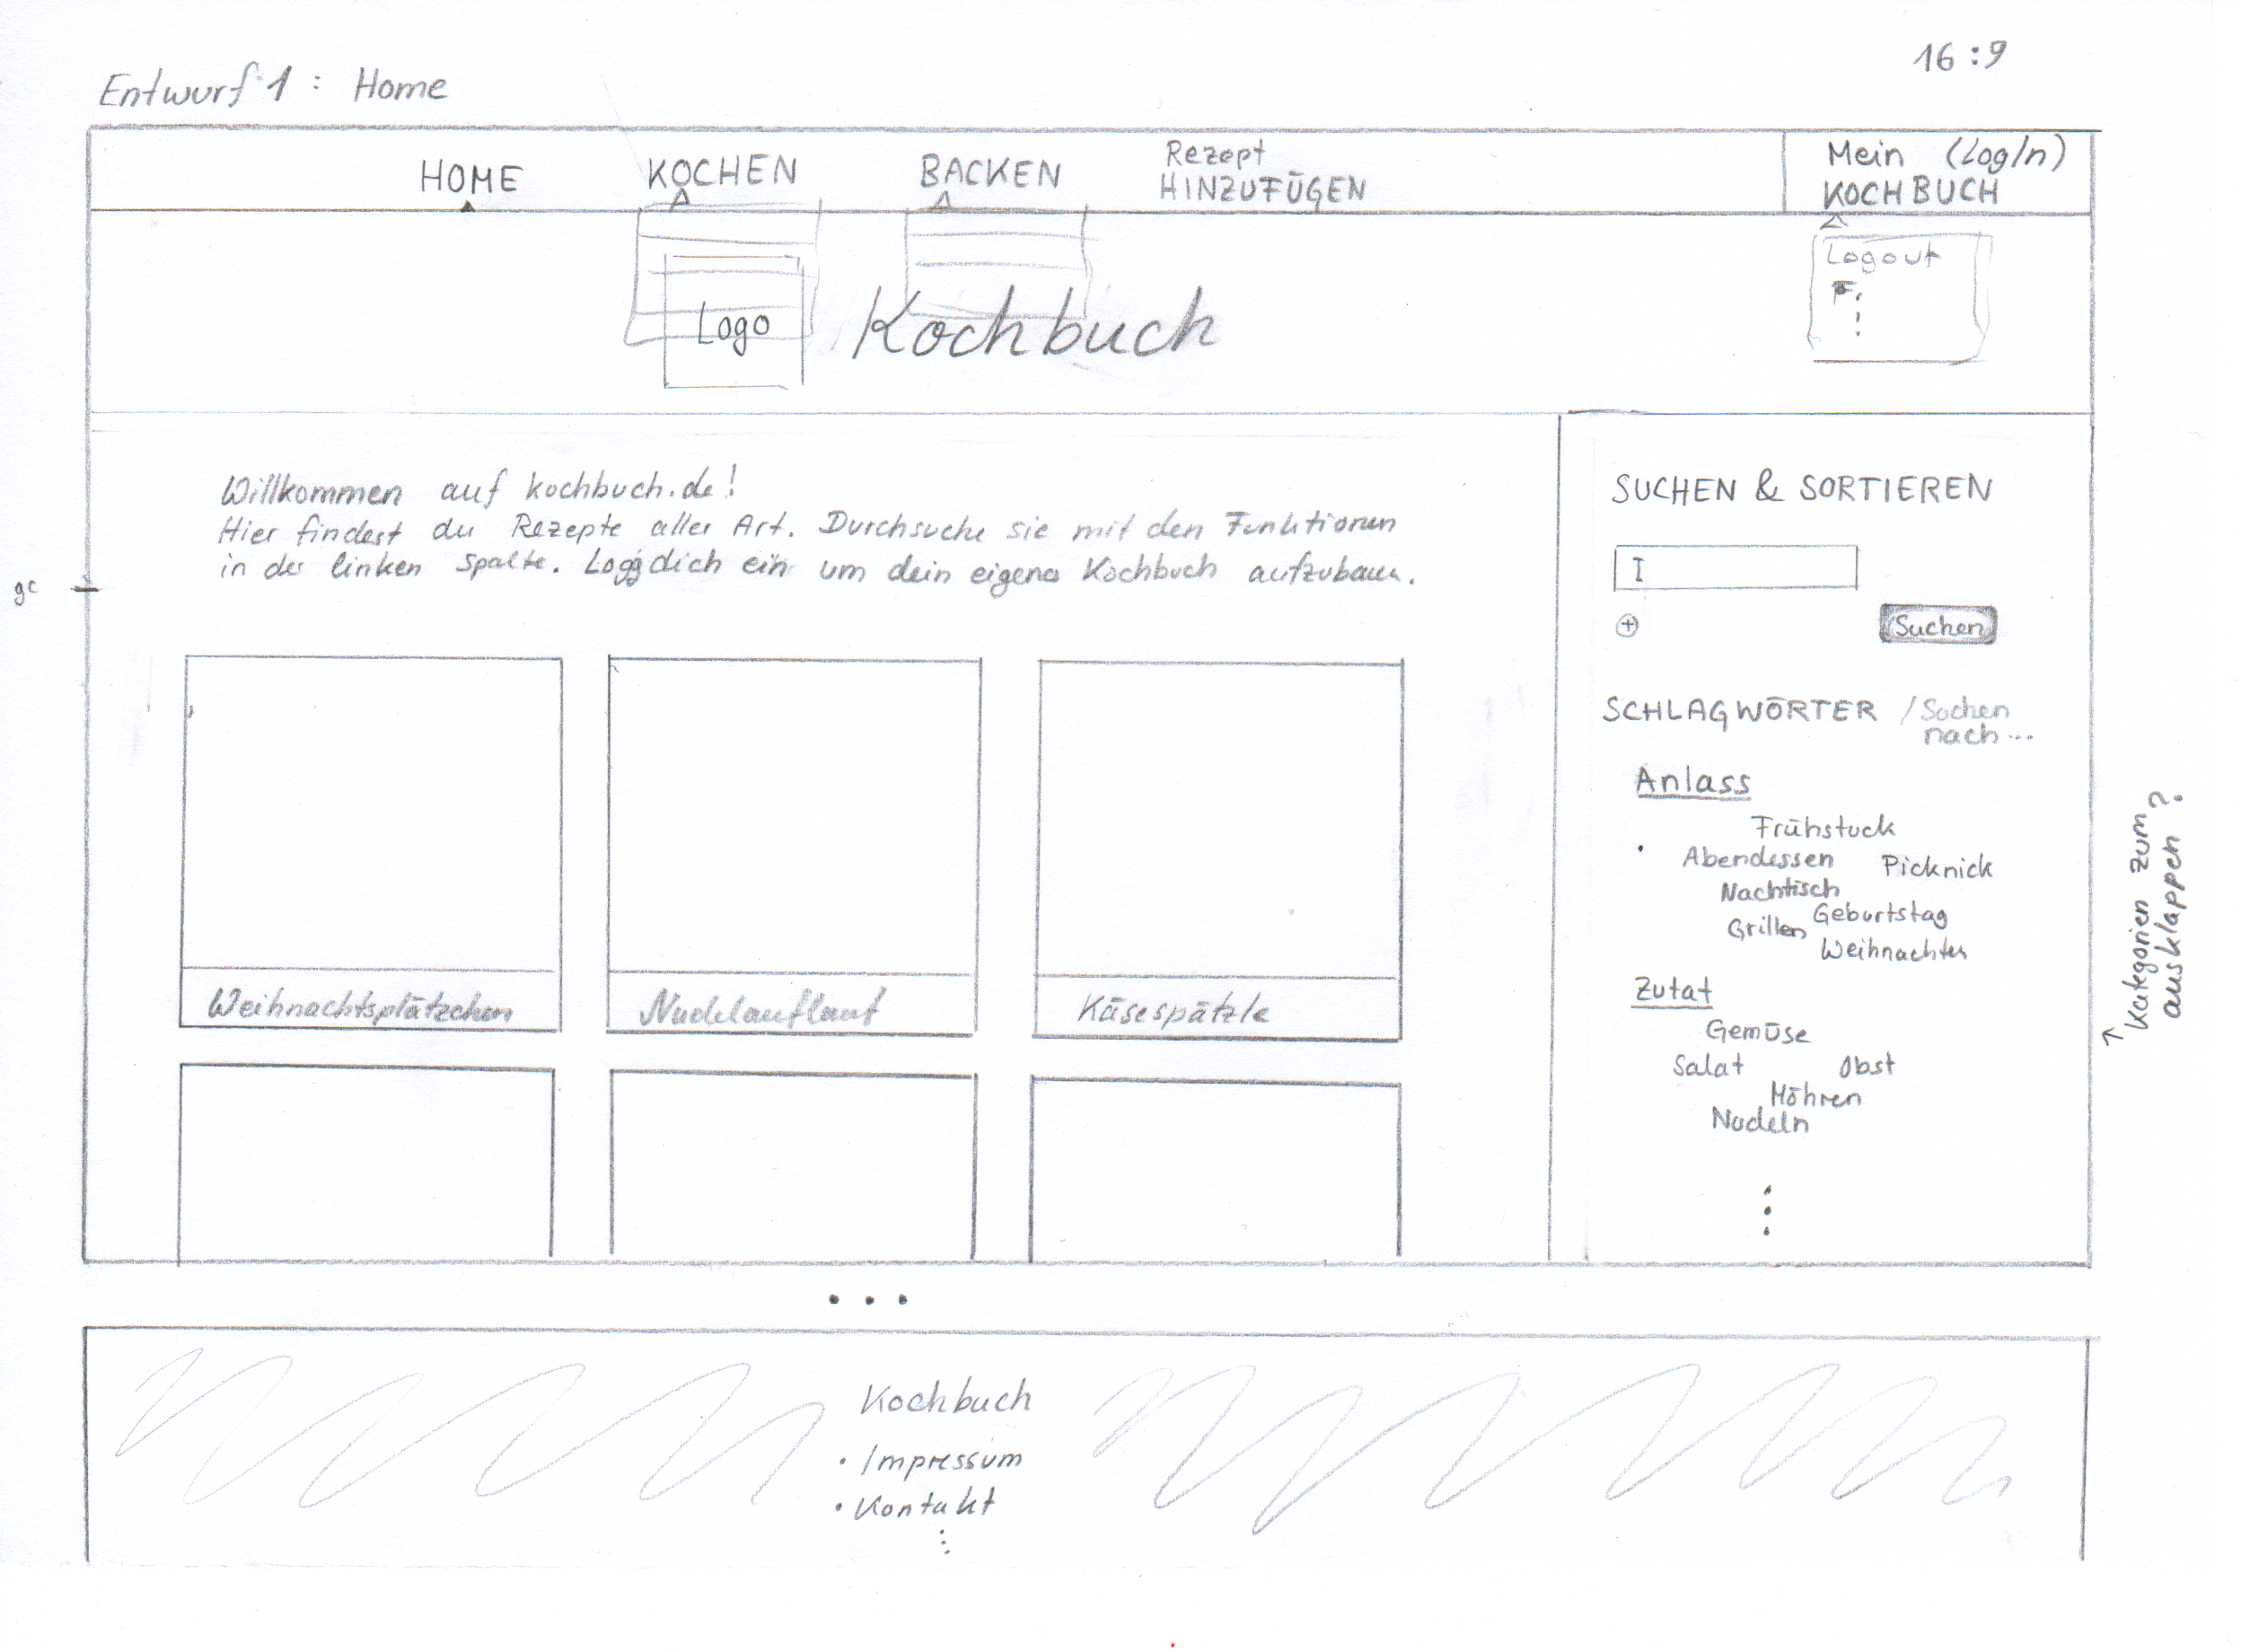
\includegraphics[scale=0.4]{Entwürfe/Tamar/entwurf1.1_home.png}
%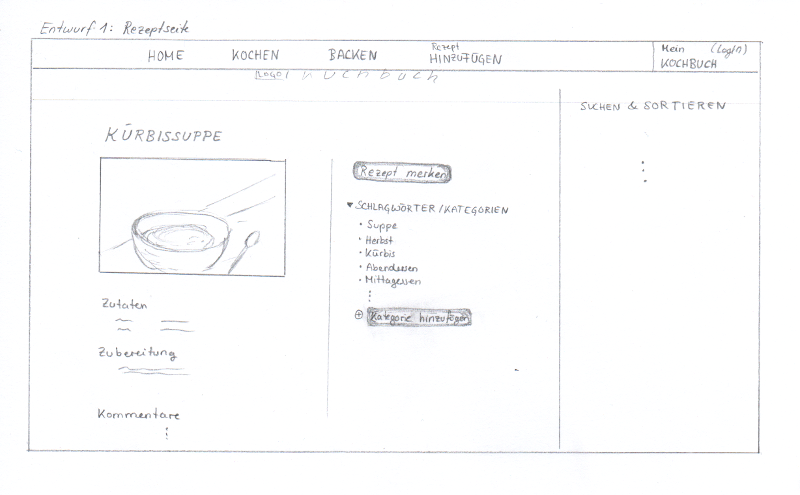
\includegraphics[scale=0.4]{Entwürfe/Tamar/entwurf1.2_rezeptseite.png}\\
%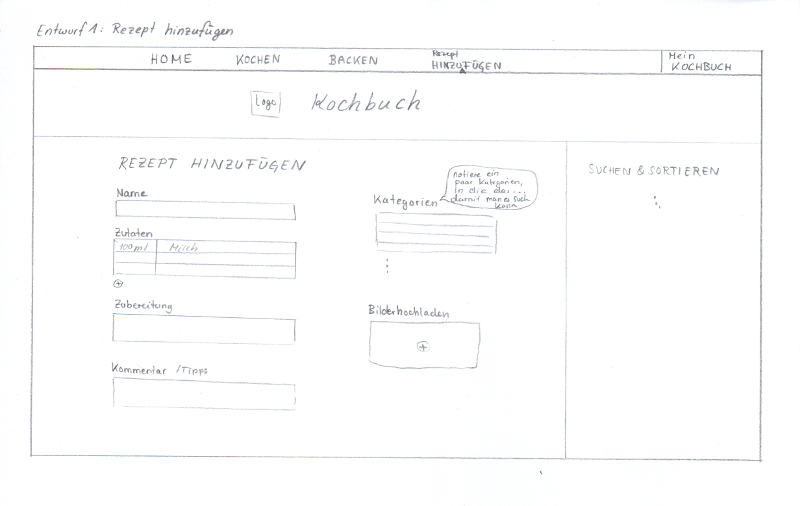
\includegraphics[scale=0.4]{Entwürfe/Tamar/entwurf1.3_hinzufügen.png}



Vorteile: \\
- klassischer Aufbau
- Suche jederzeit sichbar
- übersichtlich

Nachteile:
- Rezept hinzufügen sollte unter mein Kochbuch kommen, da es sonst nicht in die Navigationsstruktur passt
- Suchfunktion verbraucht Platz
- auf Rezeptseite muss Rezept mehr Platz einnehmen

% ------------------------------------------------------------------------------------
\section*{Entwurf 6} % Tamar 2

%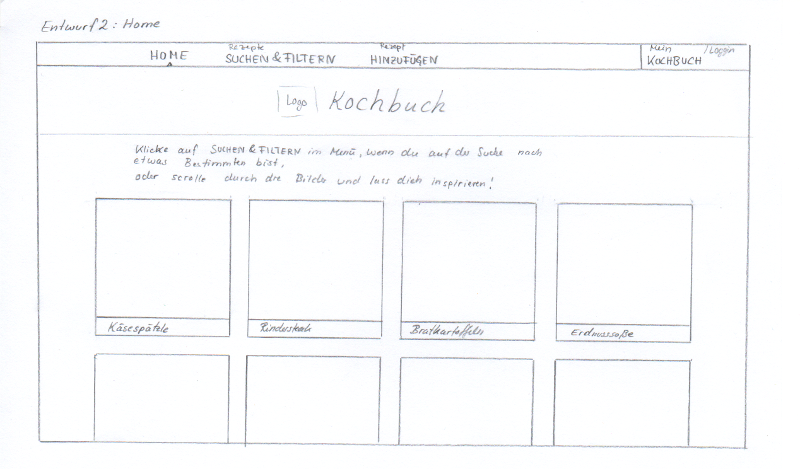
\includegraphics[scale=0.4]{Entwürfe/Tamar/entwurf2.1_home.png}
%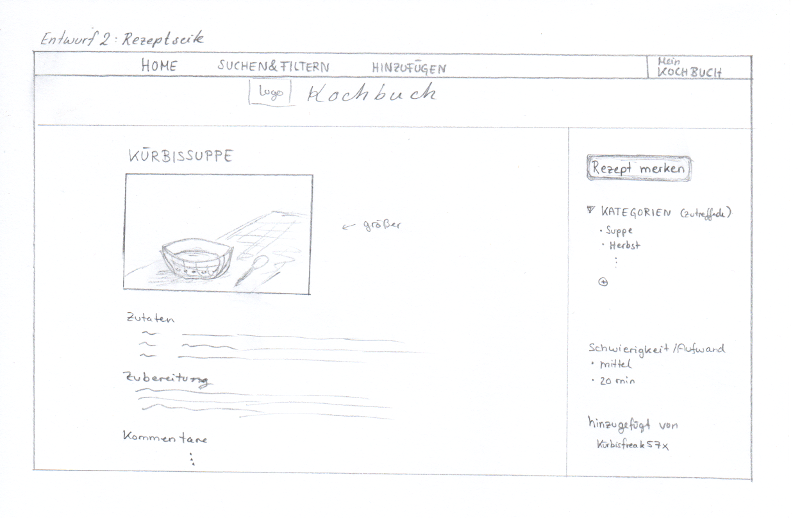
\includegraphics[scale=0.4]{Entwürfe/Tamar/entwurf2.2_rezeptseite.png}\\
%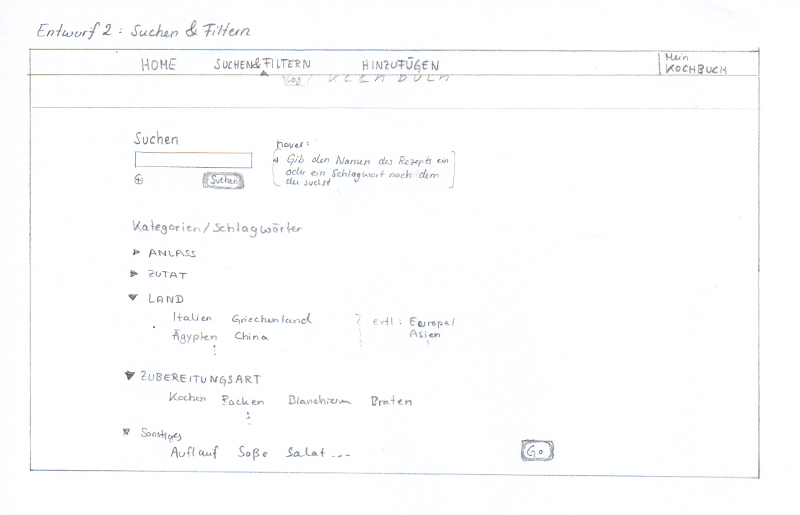
\includegraphics[scale=0.4]{Entwürfe/Tamar/entwurf2.3_filtern1.png}
%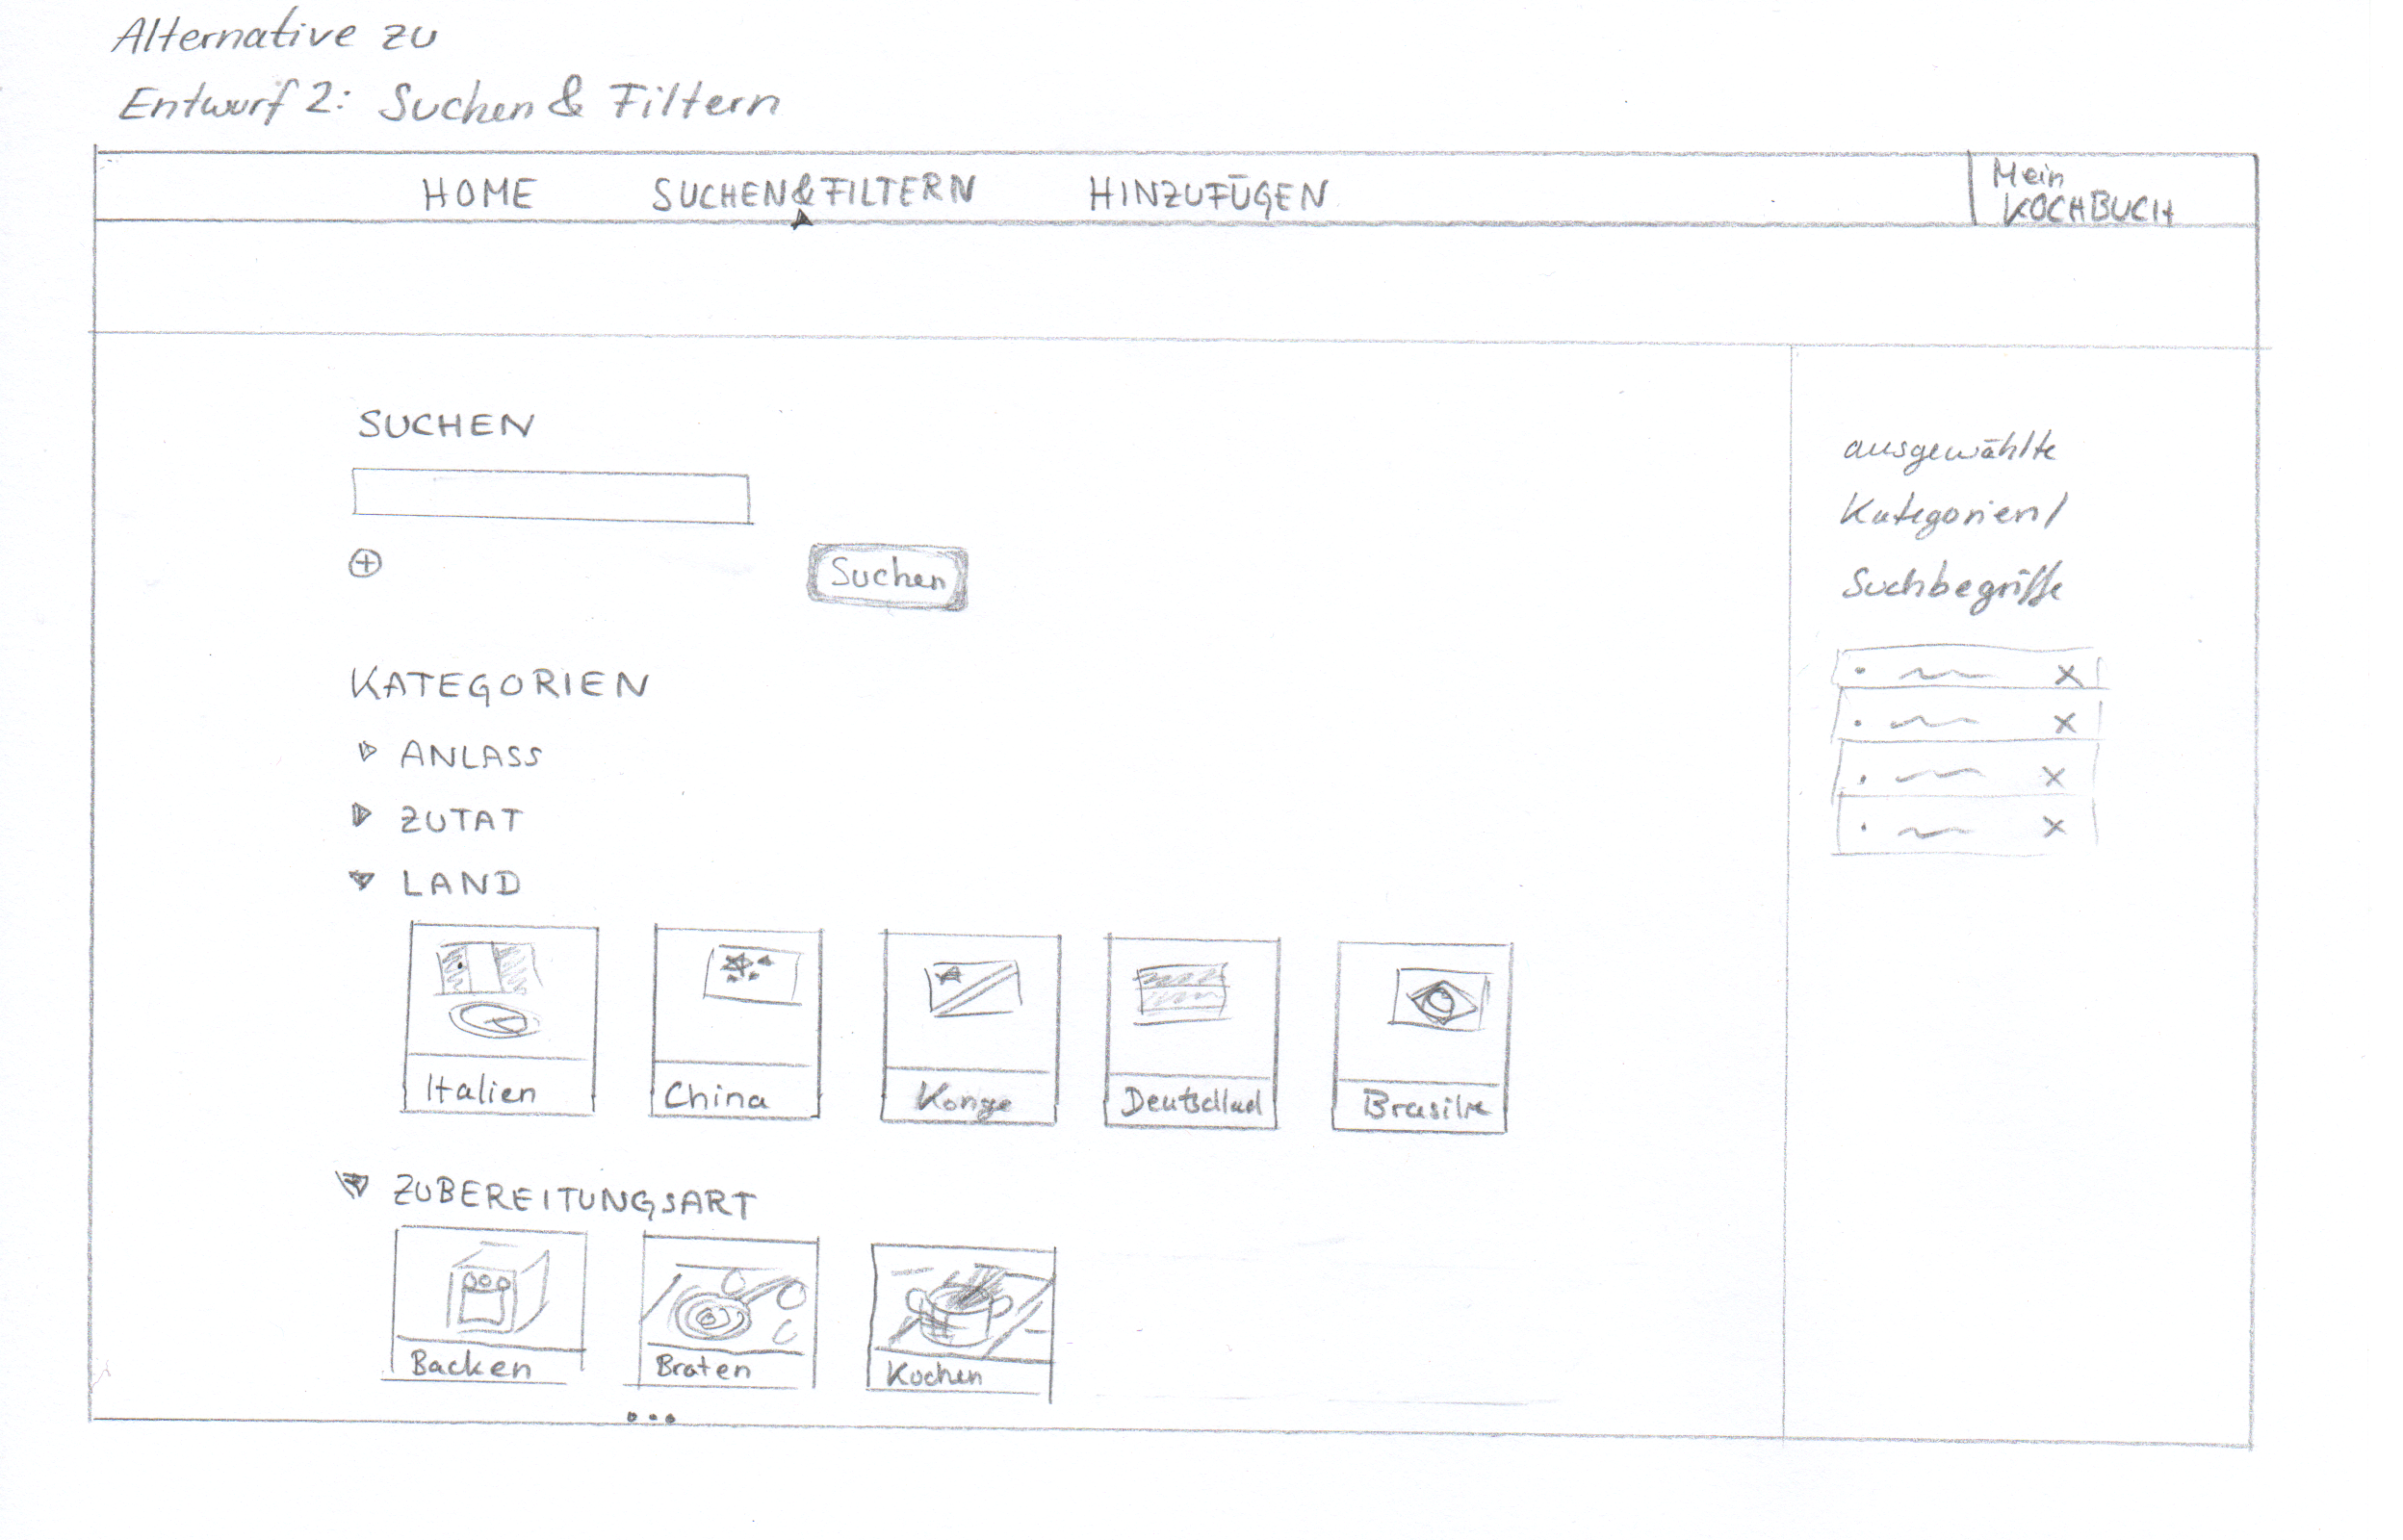
\includegraphics[scale=0.4]{Entwürfe/Tamar/entwurf2.3_filtern2.png}


Vorteile: \\
- mehr Platz
- aufgeräumter

Nachteile:
- Suche als eigene Seite hat Nachteil, dass man ausgewählte Kategorien nicht nebenher sieht.
- Suchseite zu überladen



% ------------------------------------------------------------------------------------
\section*{Planung des Prototypen}

\begin{enumerate}
 \item möglichst übersichtliches, klassisches Design um intuitives Zurechtfinden zu ermöglichen (oben rechts Login)
 \item Navigation aufgespalten:
 \begin{itemize}
  \item einerseits: horizontale Navigation stellt organisatorische Dinge dar: Metanavigation, wie Home und Profilverwaltung / persönlicher Bereich
  \item andererseits: Seitenmenü mit der Navigation durch die Rezepte (inhaltlich) \\
  Seitenmenü enthält Kategorien, nach denen Rezepte sortiert/gefiltert werden können und für "suchdominante" Menschen, und solche, die genau wissen, was sie wollen die Suchleiste
 \end{itemize}
 \item Navigation und Struktur der Webseite ist für den Nutzer ersichtlich, da auf jeder Seite Navigation an gleicher Stelle bleibt und sich eventuell dynamisch anpasst (checkboxen)
 \item Navigation nimmt nicht notwendigerweise zu viel Platz der Webseite ein, da sie eingeklappt/versteckt werden kann
 \item um seitliches Menü übersichtlich zu halten, sind die einzelnen Kategorien eingeklappt und können ausgeklappt werden
 
 \item hauptsächlicher Inhalt der Hauptseite sind die Bilder der Rezepte

\end{enumerate}


\end{document}



